\documentclass{article}
% LaTex packages 
\usepackage[utf8]{inputenc}
\usepackage{amsfonts}
\usepackage{amsmath}
\usepackage{amsthm}
\usepackage{tabto}
\usepackage{booktabs}
\usepackage{hyperref}
\usepackage{xspace}
\usepackage[utf8]{inputenc}
\usepackage{fancyvrb}
\usepackage{stmaryrd}
\usepackage{graphicx}
\usepackage{url}
\usepackage[onehalfspacing]{setspace}
% Theorems
\usepackage{pgf}
\usepackage{tikz}
\usetikzlibrary{arrows}
\usepackage{graphicx}
\usepackage{setspace}
\usepackage{amssymb}
\usepackage{mathtools}
\usepackage{tabto}
\usepackage[T1]{fontenc}
%\usepackage[a4paper,left=2cm,right=2cm,top=2cm,bottom=3cm]{geometry}
\usepackage{geometry}
 \geometry{
 a4paper,
 %total={170mm,257mm},
 %left=20mm,
 top=30mm,
 }

% This makes it possible to place a figure at the top of the page if it is the only content on the page % 
\makeatletter
\setlength{\@fptop}{0pt}
\makeatother
%

\newtheorem{thm}{Theorem}[section]
\newtheorem{cor}[thm]{Corollary}
\newtheorem{lem}[thm]{Lemma}
\newtheorem{prop}[thm]{Proposition}
\theoremstyle{definition}
\newtheorem{defn}[thm]{Definition}
\theoremstyle{remark}
\newtheorem{rem}[thm]{Remark}
\DeclarePairedDelimiter\ceil{\lceil}{\rceil}
\DeclarePairedDelimiter\floor{\lfloor}{\rfloor}
\newcommand{\eg}{e.g.,\xspace}
\newcommand{\encrypt}[1]{\ensuremath{E(#1)}\xspace}
\newcommand{\decrypt}[1]{\ensuremath{D(#1)}\xspace}

\renewcommand{\labelitemi}{$\bullet$}
\renewcommand{\labelitemii}{$\circ$}
\renewcommand{\labelitemiii}{$\cdot$}
\renewcommand{\labelitemiv}{$\ast$}

\newcommand{\btVFill}{\vskip0pt plus 1filll}

\usepackage{wrapfig}
\usepackage[font=small,labelfont=bf]{caption}

% ---- Bibliography ----

\usepackage{biblatex}
\addbibresource{references.bib}
%------------------------------------
\begin{document}
\title{Game Description}
\author{\vspace{-2.0cm} Nicola Lea Libera}
\date{May 2020}
\maketitle

\section{Abstract and Motivation}
The topic of the game is the concealment of search requests.\\
This means, given a certain topic or a concrete search request, the user has to create a search request that conceals the original request but still retrieves the desired information/ search results. \\
The motivation behind this idea is that people cam make search requests about delicate subjects without them appearing in log files.\\
With this game we want to collect data and analyze how people are hiding the search requests, e.g. are they using synonyms, or do they prefer describing objects, or are they even able to find any relevant information?. Furthermore, we can use the collected data to improve search engines. Another subject for research could be the question of how different point-systems affect the users' motivation and performance.\\
So how could this look like as a game?

\section{Game Description}
The following is a short and simple description of the basic construction and functionalities of the game. It does not cover the whole concept since it is not completely developed yet. This means some functionalities and game elements could be added or changed later in the progress of the development. \\
\\
The user is shown a topic or a precise search request that is of interest (see Figure \ref{fig:game_interface}, digit 1). He/she is then presented with a search field as used by every search engine (see Figure \ref{fig:game_interface}, digit 2). The task for him/her is now to type in a query that that retrieves as many relevant websites to the shown topic/search request as possible, e.g. the top 10 pages that would normally be shown by the search engine. The catch hereby is that the user has to conceal the shown topic. This means that he/she is not allowed to use the original search request but has to paraphrase it, use synonyms, or has to use related words/phrases. There could be two possibilities to implement this rule. It could either be only forbidden to use the words in the shown search request or there could even exist a short list with words that cannot be used (like in the game Taboo).\\
While the user is typing the query a field is shown in which he/she can see the topics and their percentage distribution of what the search engine thinks he/she is searching for (see Figure \ref{fig:game_interface}, digit 3).\\ 
Based on the abstraction of the query, the success rate and possibly the query length, points are computed (see Figure \ref{fig:game_interface}, digit 4).\\
This could be played for several rounds or within a specific time limit.\\

\begin{figure}[h]
    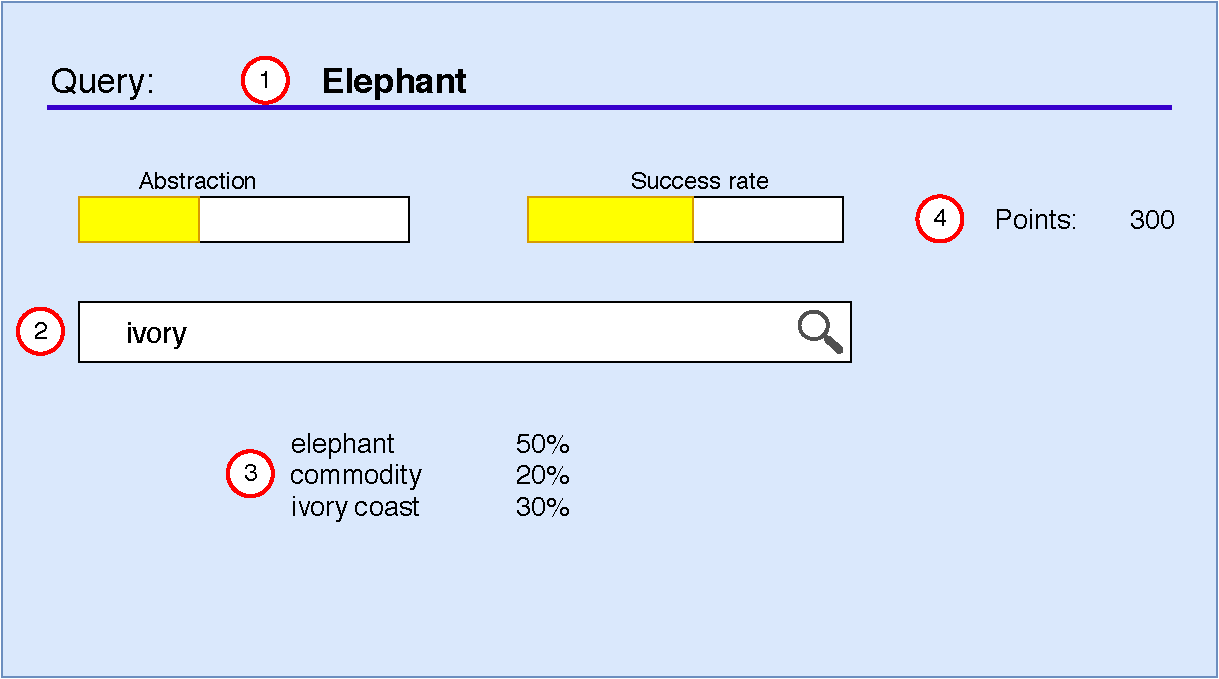
\includegraphics[width=1.0\textwidth]{images/Game.pdf}
    \caption{Rough possible interface of the game}
    \label{fig:game_interface}
\end{figure}
\btVFill
\end{document}
